\documentclass{book}
\usepackage[british]{babel}
\usepackage{tikz-feynman}

\begin{document}
 
\feynmandiagram [horizontal=a to b] {
	i1 [particle=\(b\)] -- [fermion] a -- [fermion] i2 [particle=\(\overline b\)],
	a -- [photon, edge label=\(\gamma/Z^{0}\)] b,
	f1 [particle=\(\ell^{+}\)] -- [fermion] b -- [fermion] f2 [particle=\(\ell^{-}\)],
};

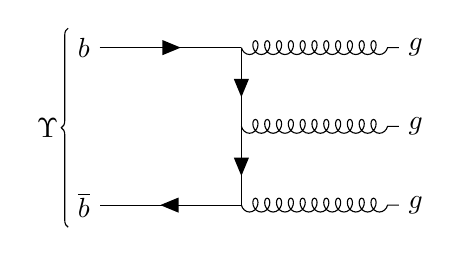
\begin{tikzpicture}
  \begin{feynman}
    \vertex (a1) {\(b\)};
    \vertex[right=2cm of a1] (a2);
    \vertex[below=1cm of a2] (a3);
    \vertex[below=1cm of a3] (a4);
    \vertex[left=1.8cm of a4] (a5){\(\overline b\)};

    \vertex[right=0cm of a2] (b1);
    \vertex[right=2cm of b1] (b2) {\(g\)};
    
    \vertex[right=0cm of a3] (c1);
    \vertex[right=2cm of c1] (c2) {\(g\)};
    
    \vertex[right=0cm of a4] (d1);
    \vertex[right=2cm of d1] (d2) {\(g\)};

    \diagram* {
      {[edges=fermion]
        (a1) -- (a2) -- (a3) -- (a4) -- (a5),
      },
      (b1) -- [gluon] (b2),
      (c1) -- [gluon] (c2),
      (d1) -- [gluon] (d2),
    };

    \draw [decoration={brace}, decorate] (a5.south west) -- (a1.north west)
          node [pos=0.5, left] {\(\Upsilon\)};
  \end{feynman}
\end{tikzpicture}

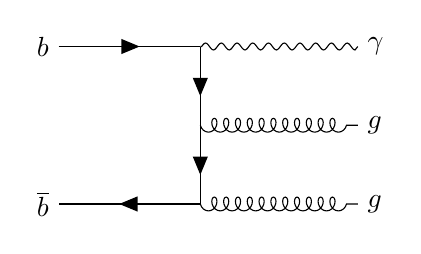
\begin{tikzpicture}
  \begin{feynman}
    \vertex (a1) {\(b\)};
    \vertex[right=2cm of a1] (a2);
    \vertex[below=1cm of a2] (a3);
    \vertex[below=1cm of a3] (a4);
    \vertex[left=1.8cm of a4] (a5){\(\overline b\)};

    \vertex[right=0cm of a2] (b1);
    \vertex[right=2cm of b1] (b2) {\(\gamma\)};
    
    \vertex[right=0cm of a3] (c1);
    \vertex[right=2cm of c1] (c2) {\(g\)};
    
    \vertex[right=0cm of a4] (d1);
    \vertex[right=2cm of d1] (d2) {\(g\)};

    \diagram* {
      {[edges=fermion]
        (a1) -- (a2) -- (a3) -- (a4) -- (a5),
      },
      (b1) -- [photon] (b2),
      (c1) -- [gluon] (c2),
      (d1) -- [gluon] (d2),
    };

  \end{feynman}
\end{tikzpicture}

\end{document}
